\label{Installationsanleitung}

Nachfolgend finden Sie eine Anleitung, wie Sie den CO$_2$-Messer in Betrieb nehmen. Bitte beachten Sie auch die zusätzlichen Hinweise. \\
Damit die Software erfolgreich vom Computer auf den Arduino geladen werden kann, müssen die folgenden Bibliotheken heruntergeladen sein:

\begin{itemize}
	\item Adafruit\_CCS811.h (Arduino-Driver für den CCS811 Gas-Sensor)
	\item SPI.h (Ermöglicht die Kommunikation mit dem Serial Peripheral Interface)
	\item Wire.h (Ermöglicht die Kommunikation über $I^2C$)
	\item LiquidCrystal.h (Zur Integration des \ac{LCD}-Displays)
	\item SD.h (Ermöglicht die Kommunikation mit dem Mikro-SD-Karten-Adapter)
\end{itemize}

\begin{figure}[!hbt]
	\centering
	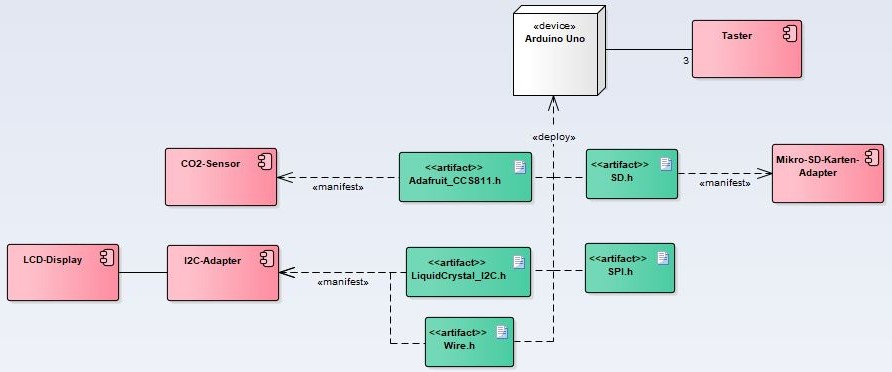
\includegraphics[width=0.9\linewidth]{Images/Diploymentdiagramm}
	\footnotesize \\Quelle: eigene Aufnahme
	\caption{Diploymentdiagramm zum Verständnis der Integration von Soft- und Hardware und deren Verbindungen}
	\label{fig:Diployment}
\end{figure}

Zunächst muss der I$^2$C-Adapter, wie in Abbildung \ref{fig:I2C} abgebildet ist, an das \ac{LCD}-Display angeschlossen werden. Achten Sie auf die Richtung der beiden Elemente. \\

\begin{figure}[!hbt]
	\centering
	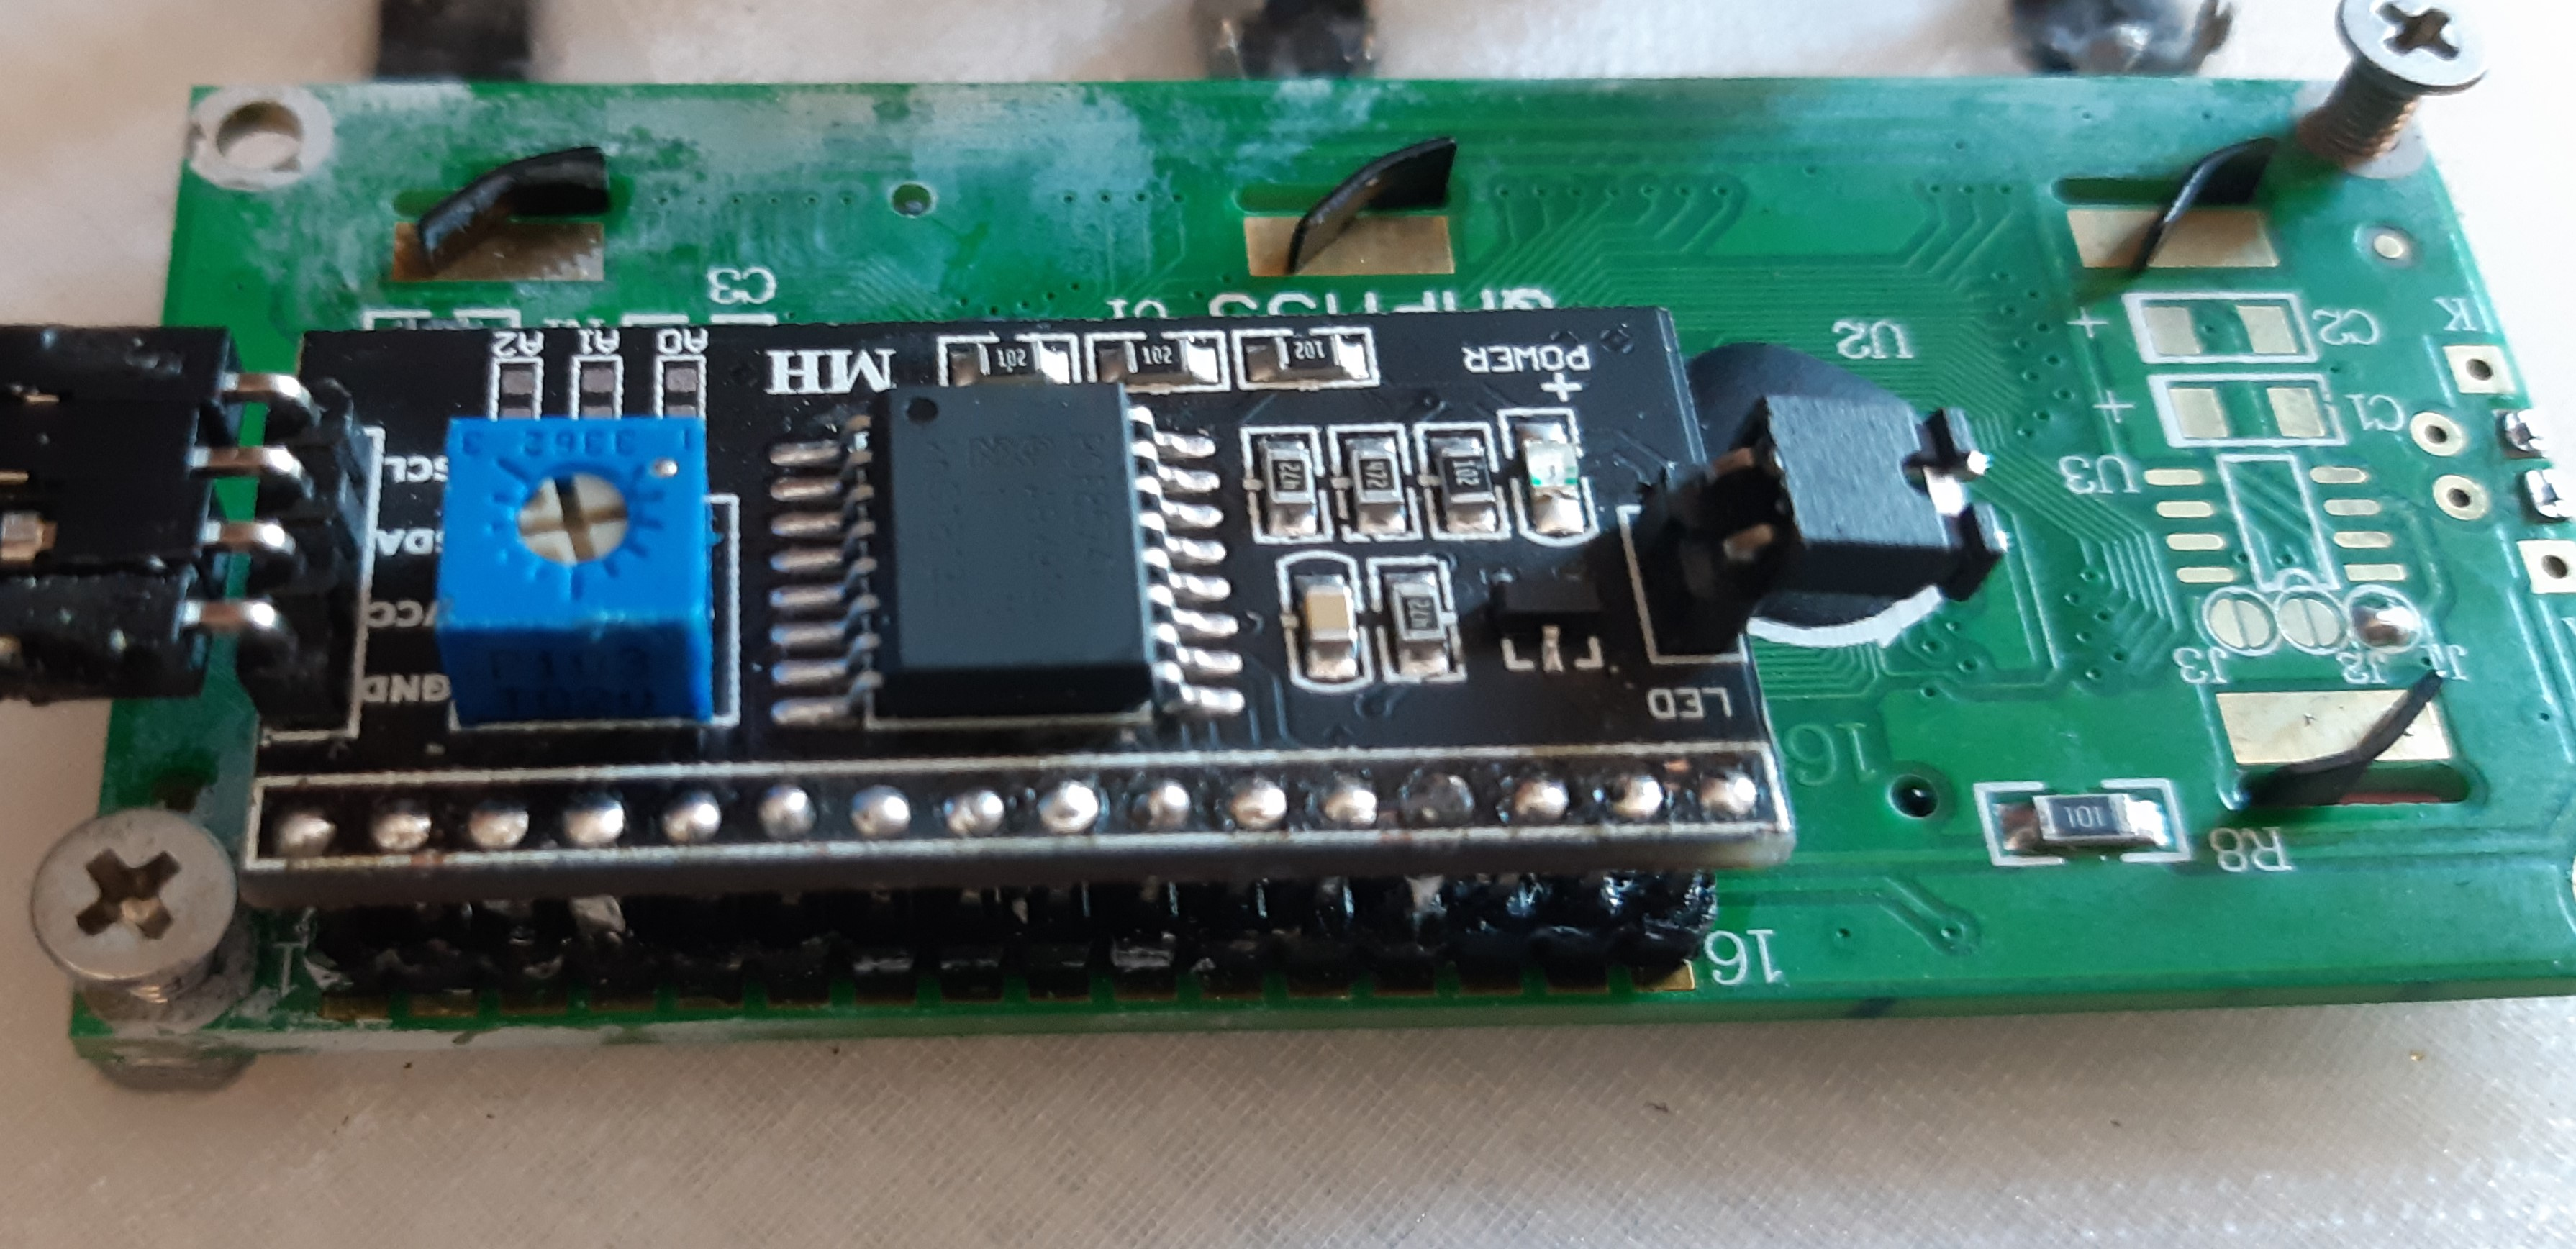
\includegraphics[width=0.6\linewidth]{Images/I2C}
	\footnotesize \\Quelle: eigene Aufnahme
	\caption{Anschluss des I$^2$C-Adapters an das \ac{LCD}-Display}
	\label{fig:I2C}
\end{figure}

In der Tabelle \ref{tab:PINs} sind alle Verbindungen zwischen den einzelnen Komponenten mit dem Arduino aufgelistet. In Abbildung \ref{fig:Layout} ist das enprechende Layout als Zeichnung zu finden. Achten Sie darauf, dass der Arduino während dieser Arbeit vom Stromnetz getrennt ist, um Kurzschlüsse zu vermeiden.

\begin{table}[!hbt]
	\centering
	\begin{tabular}{|r|l|l|l|}
		\hline
		Nummer & Bauteil & Spezifikation & Anschlusspin Arduino \\
		\hline
		1 & I$^2$C-Adapter & GND & GND \\
		 & & SDA & A1 \\
		 & & SCL & A0 \\
		\hline
		2 & \ac{LED}s & Rot & A3 \\
		 & & Gelb & A2\\
		 & & Grün & A1\\
		 & & Blau & A0\\
		\hline
		3 & Taster & Up-Button & 12 \\
		 & & Enter-Button & 13 \\
		\hline	
		4 & CCS811 & WAK & GND \\
		 & & SDA & SDA \\
		 & & SCL & SCL \\
		 & & VCC & 5V \\
		\hline
		5 & Mikro-SD-Adapter & GND & GND \\
		 & & MISO & D11 \\
		 & & MOSI & D10 \\
		 & & SCK & 9 \\
		 & & CS & 8 \\
		 & & VCC & 5V \\
		\hline
	\end{tabular}
	\captionabove{Zuordnung der Pins}
	\label{tab:PINs}
\end{table}

Auch die Vorwiderstände, welche Sie in Tabelle \ref{tab:Widerstände} sehen können, sind essentiell, um eine erfolgreiche Installation zu garantieren.

\begin{table}[!hbt]
	\centering
	\begin{tabular}{|r|l|l|}
		\hline
		Nummer & Bauteil & Vorwiderstand \\
		\hline
		1 & \ac{LED}s & 330$\ohm$ \\
		\hline
		2 & Taster & 2K$\ohm$ \\
		\hline
	\end{tabular}
	\captionabove{Verwendete Vorwiderstände innerhalb der Schaltung}
	\label{tab:Widerstände}
\end{table}

Bevor der Arduino an das Stromnetz geschlossen werden kann, kontrollieren Sie, ob sich eine Mikro-SD-Karte in dem dafür vorgesehenen Adapter befindet. Verbinden Sie anschließend das Gerät mit einer geeigneten Stromquelle. Das Menü öffnet sich und das Gerät ist installiert. Achten Sie darauf, dass der Arduino während einer Messung nicht von der Stromquelle getrennt wird. \\
